\section{Klassiska vågor}

\subsection{Principer}

\paragraph{Superposition}
Eftersom vågekvationen är linjär, interagerar vågor vid att man adderar störningarna.

\paragraph{Vågor i fas}
Två vågor är i fas om de har en fasskillnad lika med ett heltalsmultippel av $2\pi$.

\paragraph{Koherenta vågor}
Två vågor är koherenta om de har konstant fasskillnad.

\paragraph{Stående vågor}
En stående våg bildas när en våg reflekteras och interfererar med sig själv. En sådan våg har inten netto transport av energi.

\paragraph{Resonans}
Om en yttre kraft driver en svängning med en frekvens som naturligt ger stående vågor, växer amplituden obegränsat och man får stående vågor.

\paragraph{Fermats princip}
Strålgången till en klassisk våg mellan två punkter följer den snabbaste vägen.

\paragraph{Huygens' princip}
Om en våg utbrigdar sig i ett medium, kan varje punkt i mediet anses som en ny vågkälla som skickar ut en ny våg när den ursprungliga vågen träffer den givna punkten.

\paragraph{Rayleighs upplösningskriterium}
Två föremål är nätt och jämnt upplösta då interferensmaximum från det ena föremålet ligger i första sidominimum från det andra föremålet.

\subsection{Ekvationer}

\paragraph{Vågekvationen}
\begin{align*}
	\laplacian{s} = \frac{1}{c^2}\dv[2]{s}{t}
\end{align*}
Vågekvationen är fellesnämnaren för alla klassiska vågfenomen. Denna ekvation beskriver hur vågor med en väldefinierad fart $c$ propagerar i rymden över tid. $s$ är storheten som propagerar, t.ex. en tryckskillnad eller ett elektromagnetiskt fält.

\deriv
Låt störningen vara någon $f(\vect{n}\cdot\vect{r} - ct)$, der $\vect{n}$ är en enhetsvektor i samma riktning som vågens utbredning. $f$ har denna formen eftersom vågen efter en tid $t$ ser likadan ut om man beveger sig ett avstånd $ct$ i riktning av vågens utbredning. Med $u = \vect{n}\cdot\vect{r} - ct$ får man
\begin{align*}
	&\dv[2]{s}{x} = \dv{}{x}\dv{f}{u}\dv{u}{x} = n_x^2\dv[2]{f}{u}, \\
	&\vdots \\
	&\dv[2]{s}{t} = \dv{}{x}\dv{f}{u}\dv{u}{t} = c^2\dv[2]{f}{x}.
\end{align*}
Om man adderar derivatorna med avseende på rymdliga koordinater får man
\begin{align*}
	\laplacian{s} = \sum &\dv[2]{s}{x_i} = \sum n_i^2\dv[2]{f}{u} = \dv[2]{f}{u}\sum n_i^2 = \dv[2]{f}{u}
\end{align*}
då $\vect{n}$ är en enhetsvektor. Detta ger då
\begin{align*}
	\laplacian{s} = \frac{1}{c^2}\dv[2]{s}{t}.
\end{align*}

\paragraph{Dispersionsrelation för harmoniska vågor}
\begin{align*}
	\omega = ck
\end{align*}

\deriv
Ta en harmonisk våg i en dimension, på formen $Ae^{i(kx - \omega t)}$, och testa om den uppfyller vågekvationen. Då ser du att detta uppfylls under förutsättningen att dispersionsrelationen är uppfylld.

\paragraph{Harmoniska vågor}
En lösning till vågekvationen är
\begin{align*}
	s = Ae^{i(\vect{k}\cdot\vect{r} - \omega t)},
\end{align*}
och detta kommer vara basisen för vidare analys av vågfenomen. Merk att $A$ kan vara komplex och innehålla information om fasförskjutningen till vågen.

\deriv
$s$ tillfredsställar vågekvationen om dispersionsrelationen är uppfylld. Under denna förutsettning, skriv
\begin{align*}
	s = Ae^{i(\vect{k}\cdot\vect{r} - \omega t)} = Ae^{ik(\vect{n}\cdot\vect{r} - ct)},
\end{align*}
vilket är en funktion av $\vect{n}\cdot\vect{r} - ct$, som vi ville.

\paragraph{Harmonisk sfärisk våg}
\begin{align*}
	s = \frac{A}{r}e^{i(kr - \omega t)}.
\end{align*}
Faktorn $\frac{1}{r}$ kommer eftersom vågens intensitet måste vara den samma överalt.

\paragraph{Akustisk impedans}
\begin{align*}
	Z = \frac{\Delta p}{v_{\text{p}}}
\end{align*}
$v_{\text{p}}$ är partikelhastigheten i mediet.

\paragraph{Svängningar}
Om två vågor med samma amplitud men olika vågvektorer och frekvenser superponeras, uppstår en svängning. Störningen beskrivs av
\begin{align*}
	s = 2A\cos{\left(\frac{\vect{k}_{1} - \vect{k}_{2}}{2}\cdot\vect{r} - \frac{\omega_{1} - \omega_{2}}{2}t\right)}e^{i\left(\frac{\vect{k}_{1} + \vect{k}_{2}}{2}\cdot\vect{r} - \frac{\omega_{1} + \omega_{2}}{2}t\right)}.
\end{align*}
Denna består av två faktorer. Den sista faktorn är en ny våg som uppstår, och den första faktorn är en ny "amplitud" som även propagerar periodiskt. Det är denna amplituden som gör att den nya vågen varierar i intensitet, och denna variationen är upphovet till namnet.

\deriv
Om två vågor på formen $Ae^{i(\vect{k}_{1}\cdot\vect{r} - \omega_{1} t)}$ ges superpositionen av
\begin{align*}
	s &= A\left(e^{i(\vect{k}_{1}\cdot\vect{r} - \omega_{1} t)} + e^{i(\vect{k}_{2}\cdot\vect{r} - \omega_{2} t)}\right) \\
	  &= Ae^{i\left(\frac{\vect{k}_{1} + \vect{k}_{2}}{2}\cdot\vect{r} - \frac{\omega_{1} + \omega_{2}}{2}t\right)}\left(e^{i\left(\frac{\vect{k}_{1} - \vect{k}_{2}}{2}\cdot\vect{r} - \frac{\omega_{1} - \omega_{2}}{2}t\right)} + e^{i\left(\frac{-\vect{k}_{1} + \vect{k}_{2}}{2}\cdot\vect{r} - \frac{-\omega_{1} + \omega_{2}}{2}t\right)}\right) \\
	  &= Ae^{i\left(\frac{\vect{k}_{1} + \vect{k}_{2}}{2}\cdot\vect{r} - \frac{\omega_{1} + \omega_{2}}{2}t\right)}\left(e^{i\left(\frac{\vect{k}_{1} - \vect{k}_{2}}{2}\cdot\vect{r} - \frac{\omega_{1} - \omega_{2}}{2}t\right)} + e^{-i\left(\frac{\vect{k}_{1} - \vect{k}_{2}}{2}\cdot\vect{r} - \frac{\omega_{1} - \omega_{2}}{2}t\right)}\right) \\
	  &= 2A\cos{\left(\frac{\vect{k}_{1} - \vect{k}_{2}}{2}\cdot\vect{r} - \frac{\omega_{1} - \omega_{2}}{2}t\right)}e^{i\left(\frac{\vect{k}_{1} + \vect{k}_{2}}{2}\cdot\vect{r} - \frac{\omega_{1} + \omega_{2}}{2}t\right)}.
\end{align*}

\paragraph{Definition av intensitet}
Intensiteten till en våg ges av
\begin{align*}
	I = \frac{\expval{P}}{A}
\end{align*}
där $\expval{P}$ tidsmedelvärdet av den totala effekten vågen utövar och $A$ är arean av ytan vågen träffer.

\paragraph{Ljudintensitet i decibel}
\begin{align*}
	L = 10\log{\frac{I}{I_0}}
\end{align*}
$I_0$ är en referensintensitet.

\paragraph{Intensitet för superposition}
\begin{align*}
	I = I_1 + I_2 + 2\sqrt{I_1I_2}\cos{(\Delta\phi)}
\end{align*}
Två vågor med fasskillnad $\Delta\phi$ har denna intensitet när de superponeras. Märk att om vågorna ej är koherenta, blir tidsmedelvärdet av den sista termen $0$, och intensiteterna kan adderas.

\deriv

\paragraph{Stående vågor i öppen pipa}
Om en våg i en pipa reflekteras i $x = 0$ kommer den totala vågprofilen för $x < 0$ att vara
\begin{align*}
	s = 2A\cos{(\vect{k}\cdot\vect{r})}e^{-i\omega t}.
\end{align*}
Denna har noder, ställen där störningen konstant är lika med $0$, där
\begin{align*}
	\vect{k}\cdot\vect{r} = (2n + 1)\frac{\pi}{2},
\end{align*}
som i en dimension reduceras till
\begin{align*}
	x = (2n + 1)\frac{\lambda}{4}.
\end{align*}

\deriv
För en öppen pipa är trycket högare i röret än utanför, vilket gör att den akustiska impedansen i pipan är högre än utanför. I vår approximation är skillnaden extremt stor, och därmed kommer vågen att fasskiftas med $0$ och reflekteras i pipan öppning. Den totala vågprofilen blir
\begin{align*}
	s &= Ae^{i(\vect{k}\cdot\vect{r} - \omega t)} + Ae^{i(-\vect{k}\cdot\vect{r} - \omega t)} \\
	  &= Ae^{-i\omega t}(e^{\vect{k}\cdot\vect{r}} + e^{-\vect{k}\cdot\vect{r}}) \\
	  &= 2A\cos{(\vect{k}\cdot\vect{r})}e^{-i\omega t}.
\end{align*}
Det sista resultatet fås vid att hitta störningens nollställen, som endast fås om $\cos{(\vect{k}\cdot\vect{r})} = 0$.

\paragraph{Stående vågor i sluten pipa}
Om en våg reflekteras i $x = 0$ kommer den totala vågprofilen för $x < 0$ att vara
\begin{align*}
	s = 2A\sin{(\vect{k}\cdot\vect{r})}e^{-i\omega t}.
\end{align*}
Denna har noder, ställen där störningen konstant är lika med $0$, där
\begin{align*}
	\vect{k}\cdot\vect{r} = n\pi,
\end{align*}
som i en dimension reduceras till
\begin{align*}
	x = n\frac{\lambda}{2}.
\end{align*}

\deriv
För en sluten pipa träffer vågen pipans ända, där impedansen är högre än i pipan. I vår approximation är skillnaden extremt stor, och därmed kommer vågen att fasskiftas med $\pi$ och reflekteras i rörets öppning. Den totala vågprofilen blir
\begin{align*}
	s &= Ae^{i(\vect{k}\cdot\vect{r} - \omega t)} + Ae^{i(-\vect{k}\cdot\vect{r} - \omega t + \pi)} \\
	  &= Ae^{-i\omega t}(e^{\vect{k}\cdot\vect{r}} + e^{i\pi}e^{-\vect{k}\cdot\vect{r}}) \\
	  &= Ae^{-i\omega t}(e^{\vect{k}\cdot\vect{r}} - e^{-\vect{k}\cdot\vect{r}}) \\
	  &= 2iA\sin{(\vect{k}\cdot\vect{r})}e^{-i\omega t}\\
	  &= 2A'\sin{(\vect{k}\cdot\vect{r})}e^{-i\omega t},
\end{align*}
där vi har dragit $i$ in i amplituden som en fasfaktor. Det sista resultatet fås vid att hitta störningens nollställen, som endast fås om $\sin{(\vect{k}\cdot\vect{r})} = 0$.

\paragraph{Toner i öppen pipa}
I en öppen pipa med längd $L$ är endast frekvenser motsvarande
\begin{align*}
	\lambda = \frac{n}{2}L
\end{align*}
tillåtna.

\deriv
Låt $x$-axeln gå längs med vågens utbredning, som även är parallell med pipans utsträckning. Vågen skickas från $x = -L$, som är en antinod. Detta hender endast om
\begin{align*}
	\abs{\cos{(-kL)}} = 1 \\
	kL = n\pi \\
	\lambda = \frac{n}{2}L.
\end{align*}

\paragraph{Toner i sluten pipa}
I en sluten pipa med längd $L$ är endast frekvenser motsvarande
\begin{align*}
	\lambda = \frac{n}{2}L
\end{align*}
tillåtna.

\deriv
Låt $x$-axeln gå längs med vågens utbredning, som även är parallell med pipans utsträckning. Vågen skickas från $x = -L$, som är en antinod. Detta hender endast om
\begin{align*}
	\abs{\sin{(-kL)}} = 1 \\
	kL = \left(n+ \frac{1}{2}\right)\pi \\
	\lambda = \left(\frac{n}{2} + \frac{1}{4}\right)L.
\end{align*}

\paragraph{Dopplereffekt}
\begin{align*}
	f' = f_0\frac{v\pm v_{\text{o}}}{v\mp v_{\text{s}}}
\end{align*}
Detta är den fullständiga formeln som beskriver Dopplereffekten. Dopplereffekten uppstår om en mottagar rör sig relativt en källa med hastighet $v_{\text{o}}$ och källan, som skickar ut en frekvens $f_0$, även rör sig med hastigheten $v_{\text{s}}$ (alla betraktningar är här i en dimension). Mottagaren kommer då observera att vågen har en frekvens $f'$. Om de två närmar sig varandra, välj det överste tecknet.

\deriv

\paragraph{Relativistisk Dopplereffekt}
\begin{align*}
	f' = f_0\frac{1\pm\frac{v}{c}}{\sqrt{1 - \left(\frac{v}{c}\right)^2}}
\end{align*}
Denna ekvation beskriver Dopplereffekten med en relativistisk korrektion. $v$ är nu relativhastigheten mellan källa och mottagare. Igen, välj $+$ om avståndet minskar.

\paragraph{Brytningslagen}
Om en våg går från ett medium till ett annat, kommer banan ändra riktning. Om vågen träffer gränsytan med en vinkel $\theta_{\text{i}}$ relativ gränsytans normal, har man att
\begin{align*}
	\frac{\sin{\theta_{\text{i}}}}{\sin{\theta_{\text{b}}}} = \frac{c_{1}}{c_{2}}
\end{align*}
där $\theta_{\text{b}}$ är vinkeln banan har relativt gränsytan efter brytningen och vågfartens subskript anger vilket mediums vågfart det refereras till.

\deriv
Betrakta figur \ref{fig:refraction}.
\begin{figure}[!ht]
	\centering
	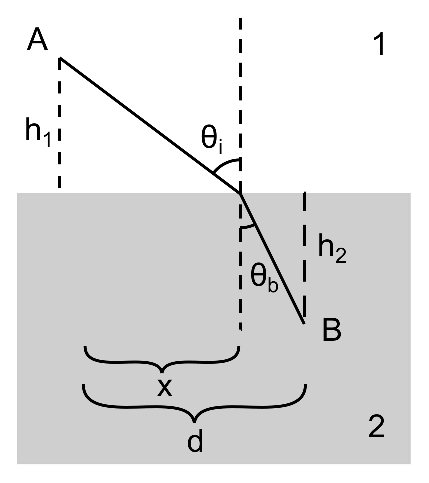
\includegraphics[scale=1]{./Images/refraction/refraction.eps}
	\caption{Illustration av brytning i en platt yta.}
	\label{fig:refraction}
\end{figure}
Tiden det tar för vågens strålgång att gå från $A$ till $B$ ges av
\begin{align*}
	t &= \frac{\sqrt{x^2 + h_1^2}}{c_1} + \frac{\sqrt{(d - x)^2 + h_1^2}}{c_2}.
\end{align*}
Derivatan med avseende på $x$ ges av
\begin{align*}
	\dv{t}{x} = \frac{x}{c_1\sqrt{x^2 + h_1^2}} - \frac{x - d}{c_2\sqrt{(d - x)^2 + h_1^2}}.
\end{align*}
Minimumet finns där derivatan är noll, vilket ger
\begin{align*}
	\frac{x}{c_1\sqrt{x^2 + h_1^2}} &= \frac{x - d}{c_2\sqrt{(d - x)^2 + h_1^2}} \\
	\frac{c_1}{c_2}                 &= \frac{\sqrt{(d - x)^2 + h_1^2}}{x - d}\frac{x}{\sqrt{x^2 + h_1^2}}.
\end{align*}
Trigonometrin ger
\begin{align*}
	\frac{c_1}{c_2} = \frac{1}{\sin{\theta_{\text{b}}}}\sin{\theta_{\text{i}}} = \frac{\sin{\theta_{\text{i}}}}{\sin{\theta_{\text{b}}}}.
\end{align*}

\paragraph{Villkor för totalreflektion}
\begin{align*}
	\theta_{\text{i}} = \arcsin{\frac{v_1}{v_2}}
\end{align*}

\deriv
Kommer direkt från brytningslagen när $\theta_{\text{i}} = \frac{\pi}{2}$.

\paragraph{Definitionen av reflektionskoefficient}
\begin{align*}
	R = \frac{I_\text{R}}{I_\text{I}}
\end{align*}
Subskriptet indikerar om det är intensiteten till den inkommande eller reflekterade vågen.

\paragraph{Definition av transmissionskoefficient}
\begin{align*}
	T = \frac{I_\text{T}}{I_\text{I}} = 1 - R
\end{align*}

\paragraph{Fassprang i gränsytor}
Om en våg går från ett medium med hög vågfart till ett med lägre, får den reflekterade vågen en fasförskjutning $\pi$. Om den går till ett medium med högre vågfart, har den reflekterade vågen samma fas.

\paragraph{Reflektionskoefficient för akustisk våg}
\begin{align*}
	R = \left(\frac{\abs{Z_1} - \abs{Z_2}}{\abs{Z_1} + \abs{Z_2}}\right)^2
\end{align*}

\paragraph{Transmissionskoefficient för akustisk våg}
\begin{align*}
	T = \left(\frac{2Z_1Z_2}{\abs{Z_1} + \abs{Z_2}}\right)^2
\end{align*}

\paragraph{Diffraktion från enkelt spalt}
\begin{align*}
	I = I_0I_0\left(\frac{\sin{\left(\frac{1}{2}ka\sin{\theta}\right)}}{\frac{1}{2}ka\sin{\theta}}\right)^2
\end{align*}
$a$ är spaltbrädden.

\deriv

\paragraph{Diffraktionsminima från enkelt spalt}
\begin{align*}
	a\sin{\theta} = m\lambda
\end{align*}

\deriv
En konsekvens formeln för intensitet vid diffraktion från enkelt spalt.

\paragraph{Diffraktion från flera spalter}
\begin{align*}
	I = I_0\frac{\sin^2{\left(\frac{1}{2}Nkd\sin{\theta}\right)}}{\sin{\left(\frac{1}{2}kd\sin{\theta}\right)}}
\end{align*}
$I_0$ är intensiteten från varje spalt, $N$ är antallet spalter, $d$ är avståndet mellan spalterna och $\theta$ är vinkeln observatören står i relativt normalen till gitteret.

\deriv
Varje källa har en vägskillnad $d\sin{\theta}$ relativt sin granne nedåt. Om man summerar vågorna får man
\begin{align*}
	s = \sum Ae^{i(kl - \omega t + (n -1)kd\sin{\theta})}
\end{align*}
för små $\theta$. Summeringen ger
\begin{align*}
	s &= Ae^{i(kl - \omega t)}\frac{1 - e^{iNkd\sin{\theta})}}{1 - e^{ikd\sin{\theta}}} \\
	  &= Ae^{i(kl - \omega t)}\frac{e^{-\frac{1}{2}iNkd\sin{\theta})}}{e^{-\frac{1}{2}ikd\sin{\theta}}}\frac{e^{\frac{1}{2}iNkd\sin{\theta}} - e^{-\frac{1}{2}iNkd\sin{\theta}}}{e^{\frac{1}{2}ikd\sin{\theta})} + e^{-\frac{1}{2}ikd\sin{\theta}}} \\
	  &= A\frac{e^{-\frac{1}{2}iNkd\sin{\theta})}}{e^{-\frac{1}{2}kd\sin{\theta}}}\frac{\sin{\left(\frac{1}{2}iNkd\sin{\theta}\right)}}{\sin{\left(\frac{1}{2}kd\sin{\theta}\right)}}e^{i(kl - \omega t)}.
\end{align*}
Den nya vågen har samma frekvens och våglängd, men en ny amplitud. Intensiteter beror på $\abs{A}^2$, vilket ger
\begin{align*}
	\frac{I}{I_0} = \frac{\sin^2{\left(\frac{1}{2}Nkd\sin{\theta}\right)}}{\sin^2{ \left(\frac{1}{2}kd\sin{\theta}\right)}}.
\end{align*}

\paragraph{Maxima vid diffraktion från flere spalter}
\begin{align*}
	d\sin{\theta} = m\lambda
\end{align*}

\deriv
Intensiteten vid flerstråleinterferens uppnår ett maximum när $\sin^2{\frac{1}{2}ikd\sin{\theta})} = 0$. Från detta kommer villkoret.

\paragraph{Första minimum vid diffraktion från en cirkulär spalt}
\begin{align*}
	\sin{\theta} = 1.22\frac{\lambda}{D}
\end{align*}
$D$ är spaltens diameter.

\paragraph{Braggs diffraktionslag}
\begin{align*}
	2d\sin{\theta} = m\lambda
\end{align*}
$d$ är separationen mellan atomplan i en kristall.

\deriv

\paragraph{Upplösning för gitter-baserat våglängdmätning}
\begin{align*}
	R = \frac{\lambda}{\Delta\lambda}
\end{align*}

\paragraph{Ljudabsorption}
\begin{align*}
	I = I_0e^{-\alpha x}
\end{align*}
Detta är ett sätt att beskriva energiförluster när vågen propagerar. $\alpha$ kallas för absorptionskoefficienten.

\paragraph{Vinkel för Mach-kon}
\begin{align*}
	\sin{\alpha} = \frac{c}{v_{\text{s}}}
\end{align*}
Om en ljudkälla rör sig med en fart $v_{\text{s}}$ som är snabbare än ljuden, kommer det bildas en så kallad Mach-kon bakom planet, där den inre vinkeln från källans bana till konens yta ges av denna ekvationen.

\deriv